%% ICSOFT 2026 -- Abstracts Track
%% Template: SCITEPRESS (SCITEPRESS.sty, article.cls, apalike.sty/bst in this dir)
%%
%% Status: English draft for co-author review
%% Source: docs/ICSOFT_2026_ABSTRACT.md
%% Pending:
%%   (1) Veronika Schwarz confirmation and affiliation
%%   (2) Veronika Schwarz affiliation confirmation (currently QAware)


\documentclass[a4paper,twoside]{article}

\usepackage{epsfig}
\usepackage{graphicx}
\usepackage{subcaption}
\usepackage{amssymb}
\usepackage{amsmath}
\usepackage{amsthm}
\usepackage{multicol}
\usepackage{pslatex}
\usepackage{apalike}
\usepackage{caption}
\usepackage{listings}
\usepackage[ruled]{algorithm2e}
\usepackage{SCITEPRESS}
\usepackage[utf8]{inputenc}
\usepackage[T1]{fontenc}

\captionsetup{font=small}

\lstdefinestyle{appendixjava}{
  language=Java,
  basicstyle=\scriptsize\ttfamily,
  numbers=left,
  numberstyle=\tiny,
  stepnumber=1,
  numbersep=6pt,
  breaklines=true,
  breakatwhitespace=false,
  columns=fullflexible,
  keepspaces=true,
  showstringspaces=false,
  tabsize=4,
  frame=single,
  literate={→}{{$\rightarrow$}}1
           {↔}{{$\leftrightarrow$}}1
           {—}{{---}}1
}

%% ---------------------------------------------------------------
\title{Verifiable Layered Architecture Visualizations
       \subtitle{Invariants for Correct Level Computation
       \\ \normalsize\textit{[Draft for co-author review]}}}

\author{
  \authorname{Johannes Weigend}
  \affiliation{Weigend AM GmbH \& Co.KG, Germany/Brazil}
  \email{johannes.weigend@weigend.de}
  \authorname{Veronika Schwarz}
  \affiliation{[Affiliation to be added]}% formerly published as Veronika Dashuber
  \email{veronika.schwarz@qaware.de}
  \authorname{Michael Philippsen}
  \affiliation{Friedrich-Alexander-Universit\"{a}t Erlangen-N\"{u}rnberg, Germany}
  \email{michael.philippsen@fau.de}
}

\keywords{software architecture visualization, layout invariants,
  layered software city, strongly connected components,
  dependency analysis, software engineering tools}

\abstract{Layered architecture visualizations communicate dependency structure
through spatial order: elements that depend on others are placed higher. If the
level-assignment pipeline is wrong, the picture can still look plausible while
misleading the viewer: a package may appear below its own classes, cyclic peer
packages may be placed on different levels, or a regular dependency may point
against the intended layer direction. Layout correctness should be the tool's responsibility, not the
reader's --- the implementation shows how hard that actually is.
\par\smallskip
Our 2021 IVAPP Best Paper, \emph{A Layered Software City for Dependency
Visualization} \cite{Dashuber2021}, introduced a city layout in which the X/Y
position of class buildings follows dependency-derived levels, while building
height encodes orthogonal metrics such as complexity or lines of code. We present Structure202, an open-source Java reference implementation
under Apache~2.0, together with a Layout Invariant Checker that verifies the
layout after every analysis run.
\par\smallskip
Correct level computation turns out not to be a single ordering problem. It requires coordinating three interdependent
constraint systems: class ordering, package containment, and level equality
within SCCs. Structure202 therefore computes two semantically
different level concepts: global architectural depth as a longest path in the
SCC-collapsed class dependency DAG, and local layout position within each
package, starting at zero and using only sibling dependencies. Highly cyclic
code bases are handled by a heuristic SCC breaker; its cut edges are not hidden
but marked as violations.
\par\smallskip
The Layout Invariant Checker verifies four postconditions: non-heuristic class
dependencies must point downward (R1); packages in a filtered package-level SCC
must share a level (R2); a container's level must equal or exceed the maximum level of its contents (R3);
and edge classifications must match the current level and SCC state (R5). A
fifth rule, R4, was deliberately retired: its generalization of R2 to the
unfiltered package graph produced false positives, because parent-child edges
and heuristic back-edges created apparent cycles between packages that are not
architectural peers (see Appendix~A). The checker distinguishes implementation bugs
from tolerated heuristic violations and emits a copy-paste-ready reproducer
block for every finding.
\par\smallskip
We will demonstrate the checker on real code bases, tracing the path from a
marked layout element to a failing reproducer test. In the 92-module
\emph{software-ekg-7} system, an R2 finding exposed a missing package-SCC
equalization step and directly triggered a pipeline fix. All four invariants
were ported to an independent Unity/.NET 3D software city and produced
byte-identical findings on shared inputs. The two-phase separation is not a design choice---no correct
level-computation pipeline can collapse the global and local questions into one
raw traversal. To our knowledge, no previous layered
architecture visualization has provided this degree of machine-checkable
self-validation; we also discuss generalization to other layered
visualization techniques.}
%% ---------------------------------------------------------------

\begin{document}

\maketitle

\vfill

\bibliographystyle{apalike}
{\small
\bibliography{icsoft2026_EN}}

%% ===================================================================
\appendix
\onecolumn

\section*{Appendix A -- Why Naive Single-Pass Does Not Work: Failure Modes}

\subsection*{The Core Problem: Three Interacting Constraint Systems}

A correct layered layout must satisfy three constraints at the same time:

\begin{enumerate}
  \item \textbf{Class constraint:} If $A \rightarrow B$ means that $A$ depends
        on $B$, then $\text{level}(A) > \text{level}(B)$.
  \item \textbf{Hierarchy constraint (R3):} A package must be placed at least
        as high as its highest contained element.
  \item \textbf{SCC constraint (R2):} All classes in a cyclic dependency group
        receive the same level; packages that form a package-level SCC must
        also share a level.
\end{enumerate}

Each constraint is individually manageable. Together they create a circular
dependency system between the levels of computation themselves, not merely
between classes.

\subsection*{Failure Mode 1: Retroactive Correction}

An algorithm iterates over classes and assigns levels. It first sees class $A$
in package $P_1$, computes $\text{level}(A)=3$, and therefore sets
$\text{level}(P_1)=3$. Later it reaches class $B$ in package $P_2$ and
discovers that $A$ and $B$ are in the same SCC and must share a level, now
$\text{level}(A)=\text{level}(B)=5$. This forces $P_1$ to be recomputed. If
$P_1$ depends on $P_3$, $P_3$ may need to move as well. A cascade follows.

In a naive single-pass implementation, however, $P_1$ and $P_3$ may already have
been finalized. SCC membership is only known after the relevant graph has been
traversed; if level assignment and SCC discovery are interleaved, the iteration
order decides whether the correction is still applied in time.

\subsection*{Failure Mode 2: Interleaved Cycle Detection Produces
Classpath-Dependent Results}

The most subtle practical failure mode occurs when cycle detection and level
computation are not separated. The algorithm traverses the class graph, assigns
levels, and handles discovered cycles on the fly, depending on which class
happens to be processed first.

Classes come from JARs. The order in which the JVM sees classes follows the
order in which they were packaged into the JAR. That order can depend on the
build tool, module order in a multi-module build, filesystem ordering on the
build server, and other implementation details. None of these orders is
semantically meaningful; none encodes architectural dependency direction.

The result is dangerous: the same source code can produce different level
layouts under different build configurations. The errors are subtle. The layout
may still look plausible, arrows may mostly point in the expected direction,
and no obvious visual break appears. Yet the precise hierarchy information is
corrupted and may remain unnoticed for a long time.

The solution is to separate the phases strictly: first compute the SCC
partition on the complete graph, then build the SCC-DAG, then assign levels.
Tarjan's algorithm computes the SCC partition in $O(V+E)$; with deterministic
input ordering, the implementation becomes reproducible and independent of
classpath traversal artifacts.

\subsection*{Failure Mode 3: Mutual Dependency Between Package and Class Levels}

Package $P_1$ is placed on the level of its highest class (R3). But the level of
that highest class depends on the classes it calls. Those classes live in
packages whose levels are again derived from their contents and dependencies.
The package graph is not available as a stable input beforehand; it is derived
from the class graph.

This mutual dependency makes a shared single pass over classes and packages
inherently unstable.

\subsection*{Failure Mode 4: The Big Lake -- SCCs Without Heuristics Collapse
the Layout}

Without a mechanism for breaking large SCCs, all members of a cyclic group must
be placed on the same level. For small cycles of two to five classes this is
acceptable. For Minecraft Forge, however, we observed a single SCC containing
4,038 classes. Without a breaker, more than 40 percent of the project would
land on one flat level at the bottom of the layout. Everything else would stand
above it, but the interesting internal structure of the core would be
invisible.

The heuristic SCC breaker solves this practical problem. It identifies back
edges, meaning dependencies that run against the natural architectural flow,
and temporarily removes them for level computation. The removed edges are
visualized as violations instead of being ignored. The layout remains honest
about architectural debt while still producing a usable hierarchy.

\subsection*{Formal Counterexample: Why a Naive Recursive Algorithm Fails}

The intuitive level-computation algorithm is a recursive DFS with memoization:

\begin{verbatim}
level(A):
  if A already computed: return level(A)
  if A has no dependencies: return 0
  return max(level(dep) for dep in A.dependencies) + 1
\end{verbatim}

For acyclic graphs this is correct and equivalent to longest-path computation
on a DAG. For cyclic graphs it fails structurally.

\textbf{Counterexample with two SCCs:}

\begin{verbatim}
SCC_1 = {A, B}, with A -> B -> A
SCC_2 = {C, D}, with C -> D -> C
Cross dependency: A -> C
\end{verbatim}

The correct levels are $\text{level}(C)=\text{level}(D)=0$ and
$\text{level}(A)=\text{level}(B)=1$.

Recursive algorithm, starting at $A$:

\begin{verbatim}
level(A)  [A "in progress", sentinel = 0]
  -> level(B)
      -> level(A): cycle detected, return 0
    B.level = 0 + 1 = 1
  -> level(C)  [C "in progress", sentinel = 0]
      -> level(D)
          -> level(C): cycle detected, return 0
        D.level = 0 + 1 = 1
    C.level = 1 + 1 = 2   <-- wrong; correct would be 0
  A.level = max(1, 2) + 1 = 3   <-- wrong; correct would be 1
\end{verbatim}

After SCC equalization, $\text{SCC}_1=\max(3,1)=3$ and
$\text{SCC}_2=\max(2,1)=2$. Both results are wrong.

The cause is that the recursive algorithm enters $\text{SCC}_2$ from the
context of $\text{SCC}_1$. The sentinel-based local cycle handling inflates the
level of $\text{SCC}_2$, and that inflated level then feeds into the
computation of $\text{SCC}_1$. The correct level of $\text{SCC}_2$, namely
zero, is only known after the graph has been collapsed into SCCs and evaluated
as an SCC-DAG.

Thus, recursive level algorithms that mix traversal, cycle handling, and level
assignment can produce traversal-order-dependent results on graphs with
interacting SCCs. In JVM-based tools, that traversal order can be influenced by
classpath and packaging order. The correct solution collapses SCCs before level
assignment: Tarjan, then SCC-DAG, then longest path.

\subsection*{The Solution: Two Semantically Different Level Concepts}

Failure modes 1 to 3 share the same root cause: trying to use one single level
concept for two different questions. Structure202 separates them:

\begin{itemize}
  \item \textbf{Phase 1} computes architectural depth: the longest path in the
        global, cycle-free SCC-DAG across all classes of the analyzed project.
  \item \textbf{Phase 2} computes local layout position inside a package: a
        zero-based ordering derived only from sibling dependencies.
\end{itemize}

Both phases use the same conceptual algorithmic shape, but on different graphs
with different constraints:

\begin{algorithm}[H]
\DontPrintSemicolon
\caption{Phase~1 -- global}
class graph\;
\Indp $\rightarrow$ Tarjan (SCCs) $\rightarrow$ SCC-DAG\;
$\rightarrow$ longest-path pass $\rightarrow$ global levels\;
$\rightarrow$ assign levels to SCC members\;
$\rightarrow$ package-level propagation upward\;\Indm
\end{algorithm}

\begin{algorithm}[H]
\DontPrintSemicolon
\caption{Phase~2 -- local, per package}
sibling graph (internal edges only)\;
\Indp $\rightarrow$ Tarjan (local SCCs) $\rightarrow$ local SCC-DAG\;
$\rightarrow$ topological pass $\rightarrow$ local layout positions\;\Indm
\end{algorithm}

Phase 1 is reproducible because SCCs are collapsed before levels are assigned.
The SCC-DAG is acyclic by construction, and longest-path computation on that
DAG is stable for the same graph.

Phase 2 intentionally ignores external dependencies. If package \texttt{ui}
depends on \texttt{domain} and \texttt{domain} depends on \texttt{persistence},
external edges would otherwise pull many siblings into global levels and make
their local structure unreadable. Phase 2 sees only sibling relationships and
produces a package-local ordering that is independent of the global
architectural depth.

The central argument is that no single level concept can serve both purposes
well. A purely global level is often visually useless inside a package; a
purely local level has no architectural meaning. The explicit separation
enables a layout that is both structurally correct and readable.

\begin{table}[h]
\centering
\small
\begin{tabular}{lll}
\hline
 & \textbf{Phase 1} & \textbf{Phase 2} \\
\hline
\textbf{Meaning}      & Architectural depth in SCC-DAG          & Visual position among siblings \\
\textbf{Scope}        & Global --- all project classes          & Local --- children of one package \\
\textbf{Zero point}   & Leaf classes $= 0$; grows with depth    & Always $0$ for the lowest sibling \\
\textbf{Cycles}       & Eliminated by SCC collapse             & Handled by local Tarjan \\
                      & before level assignment                 & \\
\textbf{Value range}  & Project-dependent; can reach hundreds   & Small integers (sibling count $-1$) \\
\hline
\end{tabular}
\caption{The two level concepts computed by Structure202.}
\end{table}

The implemented invariants R1, R2, R3, and R5 are machine-checkable
postconditions for exactly this pipeline separation. The fact that the checker
found a real R2 bug in \emph{software-ekg-7} shows that the rules are not
trivial to satisfy, even for the authors of the algorithm.

\subsection*{Implementation: The Complete Pipeline}

The conceptual two-phase structure expands into the following concrete
implementation steps.

\begin{algorithm}[H]
\caption{Phase~1 -- Global Level Computation (\texttt{LevelCalculator})}
\DontPrintSemicolon
\textbf{Step~1:} Create class objects \hfill (all levels $\gets 0$)\;
\textbf{Step~2:} Create package objects \hfill (all levels $\gets 0$)\;
\BlankLine
\textbf{Step~3:} Compute class levels\;
\Indp
  $\rightarrow$ Tarjan on class graph\;
  $\rightarrow$ SCCBreaker: identify back edges (iterates until no SCC $\ge 3$ remains)\;
  $\rightarrow$ Remove back edges $\rightarrow$ filtered class DAG\;
  $\rightarrow$ Condense filtered DAG into SCC super-nodes\;
  $\rightarrow$ Single longest-path pass on condensed DAG\;
  $\rightarrow$ Assign SCC level to all members (equalization implicit)\;
\Indm
\BlankLine
\textbf{Step~4:} Package level $\gets \max(\text{level of contained classes})$\;
\BlankLine
\textbf{Step~5a:} Lift parent package levels --- initial bottom-up pass:\;
\Indp sort packages deepest-first; $\text{parent.level} \gets \max(\text{child.level})$\;\Indm
\BlankLine
\textbf{Step~5b:} Order packages by cross-package dependencies --- DFS post-order pass:\;
\Indp DFS post-order on simple cross-package graph; $\text{pkg.level} \gets \max(\text{dep.level})+1$\;\Indm
\BlankLine
\textbf{Step~5c:} Equalize package SCCs (R2) and re-lift parents to a fixpoint:\;
\Indp repeat Tarjan-SCC max equalization and parent lift until no package level changes\;\Indm
\BlankLine
\textbf{Step~6:} Set reverse dependencies (dependents)\;
\end{algorithm}

After Step 3, level is no longer a property of an individual class alone. It is
the level of the SCC node to which the class belongs, measured as the longest
path in the cycle-free quotient graph. That graph covers all classes of the
analyzed project, across packages. Cycles do not influence level assignment
internally because they have already been collapsed before longest-path
computation. This is the fundamental difference from naive recursive
approaches, and it is the reason why Phase 2 must be a separate computation.

\begin{algorithm}[H]
\DontPrintSemicolon
\caption{Phase~2 -- Local Visualization Positions (\texttt{DistrictRowLevelCalculator}, recursively per package)}
\textbf{for each} package $P$:\;
\Indp
  \textbf{Step~1:} Collect subtree classes per sibling\;
  \Indp (class: $\{\text{itself}\}$;\enspace package: all classes recursively)\;\Indm
  \BlankLine
  \textbf{Step~2:} Build sibling graph via distinct-target counting:\;
  \Indp
    $\mathrm{count}_{A \to B} = |\{\,c \in \mathrm{subtree}(B) \mid c \in \mathrm{deps}(A)\,\}|$\;
    $\mathrm{count}_{B \to A} = |\{\,c \in \mathrm{subtree}(A) \mid c \in \mathrm{deps}(B)\,\}|$\;
    add edge $A \rightarrow B$ \textbf{if} $\mathrm{count}_{A \to B} > \mathrm{count}_{B \to A}$\;
  \Indm
  \BlankLine
  \textbf{Step~3:} Tarjan $\rightarrow$ local SCC-DAG $\rightarrow$ longest-path $\rightarrow$ local levels\;
  \textbf{Step~4:} Apply levels to all siblings\;
  \textbf{Step~5:} Recurse into child packages\;
\Indm
\end{algorithm}

Step~5c is intentionally a monotone fixpoint, not an arbitrary bounded loop.
The R2 equalization step can lift a package-SCC member to the maximum level of
its peer group. A subsequent parent lift can then raise a parent package that is
itself part of another package-SCC, which may require one more R2 equalization.
Both operations only raise levels and only copy existing maximum levels; no rule
creates an unbounded sequence of fresh levels. Since the number of packages and
level values is finite, the iteration terminates when neither operation changes
any package level. The result is the least fixpoint satisfying package-SCC
equality (R2) and container dominance (R3) after cross-package ordering.

A single-pass implementation is possible, but only by moving complexity earlier:
one must first build a combined constraint graph containing the filtered
package-dependency constraints and the child-to-parent containment constraints,
condense that graph into components, initialize each component with the maximum
level of its members, and then run a single topological max-propagation pass on
the resulting component DAG. The implemented fixpoint keeps these concerns
explicit and is validated by the same R2/R3 invariants.

The term ``two phases'' refers to the conceptual separation between global
architectural depth and local layout position, not to the raw number of
implementation steps. Phase 1 is an ordered pipeline with one monotone package
fixpoint. Phase 2 is an independent local computation.

\subsection*{R2 Fix in \emph{software-ekg-7}: Visual Evidence}

The \emph{software-ekg-7} case is the concrete failure that forced the
monotone Step~5c fixpoint. Before the fix, the city view still looked plausible:
the package rectangles and dependency streets formed a readable layout, and no
single visual element made the pipeline defect obvious. The metrics panel,
however, exposed the inconsistency: 167 dependency violations were reported and
the maximum architectural level had inflated to 160. After the R2 fixpoint was
introduced, the same input produced zero violations and a maximum level of 18.
The number of classes, packages, dependencies, cyclic classes, and tests stayed
constant; the change is therefore attributable to level propagation, not to a
different input model.

\begin{figure}[h]
  \centering
  \begin{subfigure}{0.49\textwidth}
    \centering
    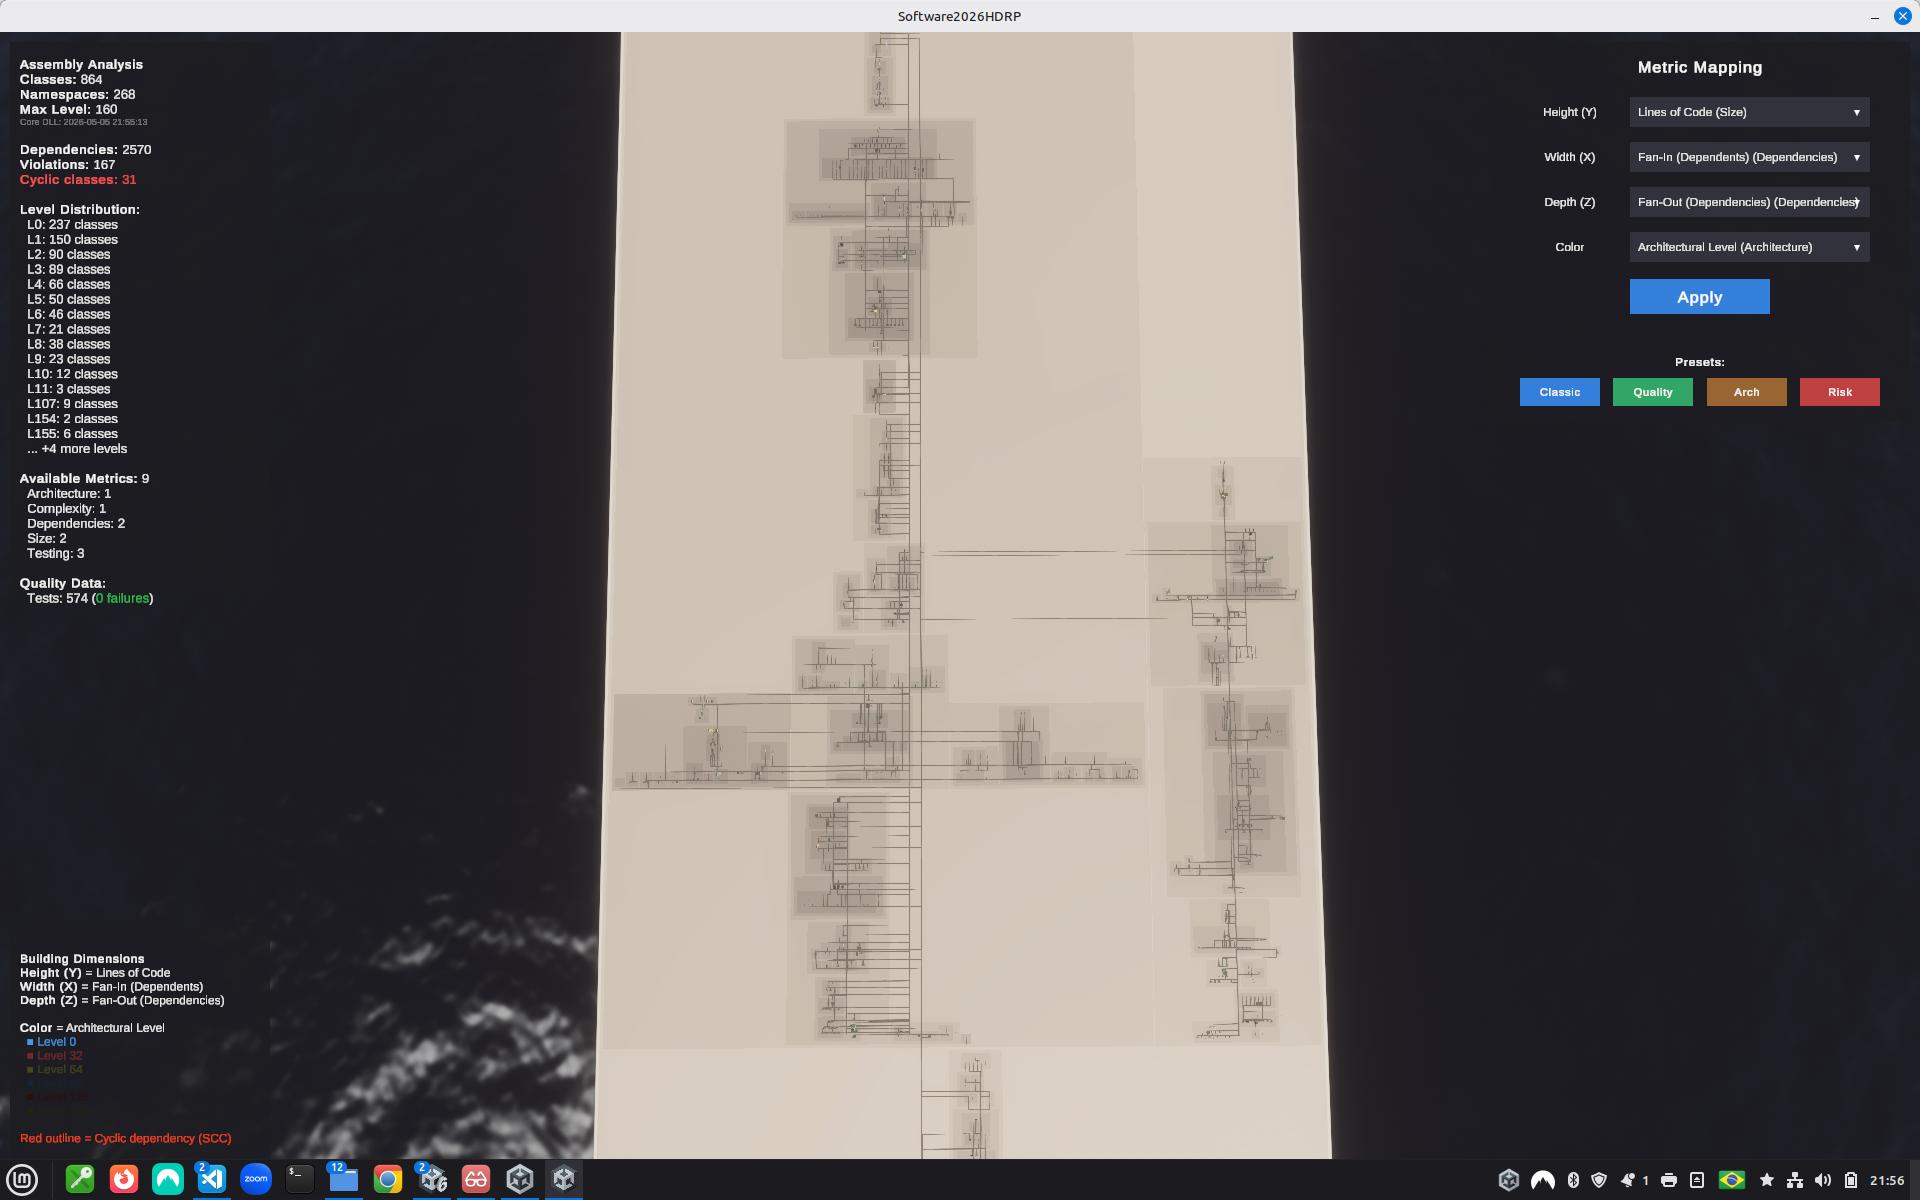
\includegraphics[width=\linewidth]{figures/SW-EKG7-Baseline.png}
    \caption{Before the R2 fix: the full city view looks plausible, but the
    metric panel reports 167 violations and MaxLevel 160.}
  \end{subfigure}
  \hfill
  \begin{subfigure}{0.49\textwidth}
    \centering
    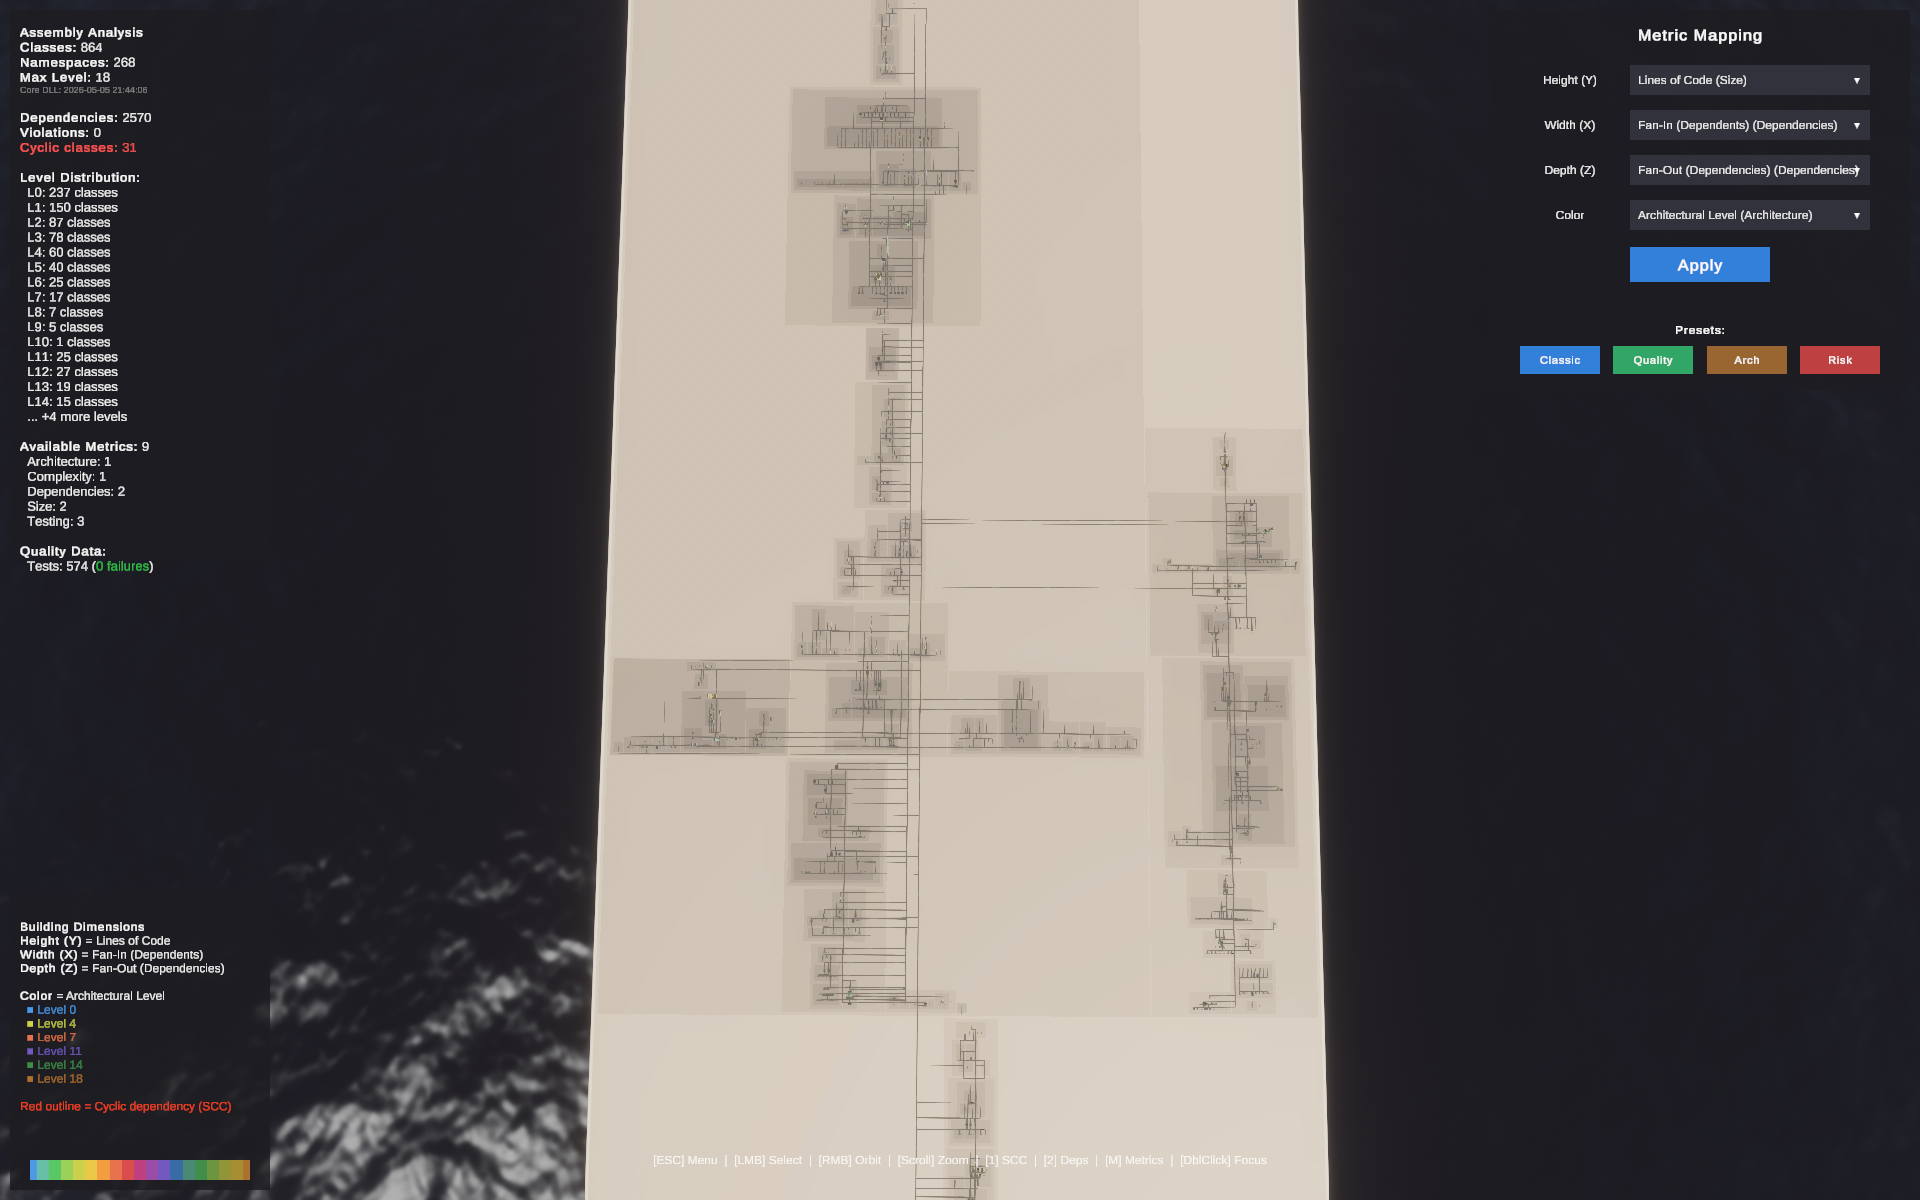
\includegraphics[width=\linewidth]{figures/SW-EKG7-Nach-Level-Fix-per-Constraint-Analyses.png}
    \caption{After the monotone R2 fixpoint: the same analyzed system reports
    zero violations and MaxLevel 18.}
  \end{subfigure}
  \caption{Full-screen before/after screenshots of the \emph{software-ekg-7}
  software city. The visible city changes only subtly; the level metrics reveal
  the correction.}
  \label{fig:swekg7-before-after}
\end{figure}

\begin{figure}[h]
  \centering
  \begin{subfigure}{0.31\textwidth}
    \centering
    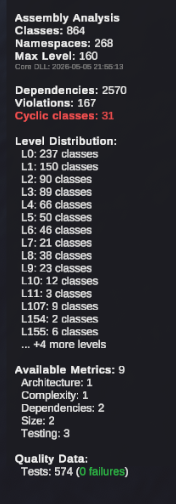
\includegraphics[width=\linewidth]{figures/Vor-Constraintfix.png}
    \caption{Before: 167 violations, MaxLevel 160.}
  \end{subfigure}
  \hspace{0.08\textwidth}
  \begin{subfigure}{0.31\textwidth}
    \centering
    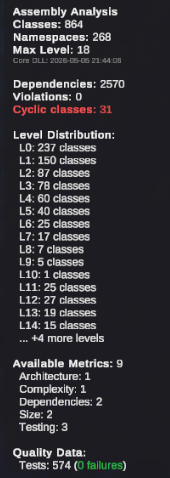
\includegraphics[width=\linewidth]{figures/Nach-Constraintfix.png}
    \caption{After: zero violations, MaxLevel 18.}
  \end{subfigure}
  \caption{Cropped metric panels from Figure~\ref{fig:swekg7-before-after}.
  These panels are the clearest user-visible symptom of the R2 propagation
  defect and its fix.}
  \label{fig:swekg7-metrics}
\end{figure}

The invariant checker closes the loop from visual symptom to reproducible
algorithm defect. Figure~\ref{fig:invariant-dialogs} shows two dialog outputs
from the checker: an R2 package-SCC equal-level finding and an R3 container
dominance finding. The R2 finding is precisely the class of defect addressed by
the fixpoint in Step~5c; R3 demonstrates why the parent lift must remain part of
the same monotone constraint system rather than being treated as an unrelated
post-processing step.

\begin{figure}[h]
  \centering
  \begin{subfigure}{0.49\textwidth}
    \centering
    
\includegraphics[width=\linewidth]{\detokenize{figures/Invariant Finding R2.png}}
    \caption{R2 report: packages in a filtered package-SCC are placed on
    different levels.}
  \end{subfigure}
  \hfill
  \begin{subfigure}{0.49\textwidth}
    \centering
    
\includegraphics[width=\linewidth]{\detokenize{figures/Invariant Finding R3.png}}
    \caption{R3 report: a parent package is below one of its contained
    packages.}
  \end{subfigure}
  \caption{Invariant-checker dialogs. Findings are reported as algorithm-bug
  candidates with a copy-paste-ready reproducer block, which makes the visual
  failure traceable to concrete level-pipeline constraints.}
  \label{fig:invariant-dialogs}
\end{figure}

\subsection*{R4: A Retired Rule and What It Teaches}

An early version of the invariant checker contained R4:

\begin{verbatim}
Cyclic child packages must share a level.
\end{verbatim}

The rule sounds reasonable and is correct in simple cases. In practice it
failed because the raw package graph contains relationships that should not be
interpreted as peer-level architectural cycles:

\begin{itemize}
  \item \textbf{Parent-child edges} create apparent bidirectional relationships
        because a parent contains its children and children belong to their
        parent. Without filtering, many parent/child pairs look cyclic.
  \item \textbf{SCCBreaker back edges} connect packages that are not
        necessarily architectural peers. A rule that includes these edges
        equalizes the wrong candidates.
  \item \textbf{Shared class SCCs} can make two packages appear
        package-dependent without representing a true structural peer
        relationship.
\end{itemize}

R4 was replaced by R2, which expresses the same intention on the correct
filtered graph. R2 removes heuristic back edges, intra-subtree edges, and edges
caused by shared class SCCs before running Tarjan on the remaining package
graph.

Specifying invariants for a three-level constraint system turns out to be
non-trivial in its own right. The checker therefore provides a second safety
net: it not only tests the implementation against the rules, but also exposes
when the rules themselves are too broad or too coarse. False positives force the rule to
become more precise. The later R2 finding in \emph{software-ekg-7} shows that
the refined rule was precise enough to distinguish real pipeline bugs from
apparent ones.

\subsection*{Interactive Debt Navigation: Top-Cut-Targets}

For interactive debt resolution, a \emph{Top-Cut-Targets} panel lists the
specific method calls that appear most frequently across the cut edges
identified by the SCCBreaker. For each method, the panel shows the involved
caller classes; a \emph{Cut All} context menu removes all associated edges at
once. This closes the gap between a visual diagnosis --- a red edge in the city
layout --- and a targeted refactoring action: the user sees which concrete call
must be removed or inverted to dissolve the most tangles with the least effort.

\subsection*{Relation to Feedback Arc Set Heuristics}

Failure Mode 4 is an instance of the Minimum Feedback Arc Set problem: remove a
minimal set of directed edges so the graph becomes acyclic. The problem is
NP-hard \cite{Karp1972}, so any practical polynomial-time implementation must
use a heuristic or approximation.

A well-known related heuristic is due to Eades, Lin, and Smyth \cite{Eades1993}.
It orders nodes according to the difference between outgoing and incoming
degree, then classifies edges that point backward in the resulting sequence as
feedback edges. The intuition is similar to Structure202: high out-degree
suggests a higher-level element; high in-degree suggests a foundational
element.

Structure202 uses a deliberately simpler variant: a direct normalized score per
node,

\[
  \frac{\text{outDegree} - \text{inDegree}}
       {\max(1, \text{outDegree} + \text{inDegree})}.
\]

Edges from lower-ranked to higher-ranked nodes are classified as back-edge
candidates. This is easier to implement and sufficient for software dependency
graphs, where the heuristic reflects architectural intuition rather than
claiming mathematical optimality.

The important distinction is transparency. Many tools break cycles implicitly,
but Structure202 classifies heuristic cut edges explicitly. They are marked as
\texttt{VIOLATION}, rendered in red, and known to the invariant checker. This
makes algorithmic defects separable from tolerated heuristic artifacts.

\section*{Summary}

Correct level computation for layered architecture visualizations requires
satisfying three interacting constraint systems simultaneously: class dependency
ordering, package containment (R3), and SCC level equality (R2). No single
traversal pass can satisfy all three; the failure modes documented above are
structural, not accidental.

Structure202 resolves this by separating two semantically distinct level
concepts: global architectural depth, computed as the longest path in the
SCC-collapsed class dependency DAG, and local layout position within a package,
derived exclusively from sibling dependencies. The Layout Invariant Checker
verifies four machine-checkable postconditions (R1, R2, R3, R5) after every
analysis run and emits copy-paste-ready reproducer blocks for each finding.

The \emph{software-ekg-7} case demonstrates that the checker catches defects
invisible to visual inspection: a plausible city layout reported 167 violations
and a maximum architectural level of 160; after the R2 equalization step was
corrected, the same input produced zero violations and a maximum level of~18,
with no change to the analyzed source code.

\clearpage

\section*{Appendix B -- LevelCalculator Reference Implementation}

The following source excerpt is the complete Java implementation of the global
level pipeline discussed above. It includes the monotone Step~5c fixpoint that
replaced the former hard-coded iteration bound.

\lstinputlisting[style=appendixjava]{../../analyzer/src/main/java/de/weigend/s202/domain/LevelCalculator.java}

\section*{Open Points Before Submission}

\begin{itemize}
  \item Confirm Veronika Schwarz as co-author and verify affiliation (e-mail: veronika.schwarz@qaware.de).
  \item Keep the submission abstract to one page in the INSTICC template.

\end{itemize}

\end{document}
